% encoding: utf8
% !TEX encoding = utf8
% !TeX spellcheck = pl_PL


\documentclass[12pt,a4paper]{article}
\usepackage[margin=0.5in]{geometry}
\usepackage{amsmath}
\usepackage{amssymb}
\usepackage[english,polish]{babel}
\usepackage{cite}
\usepackage{graphicx}
\usepackage{hyperref}
\usepackage[utf8]{inputenc}
\usepackage{listings}
\usepackage{polski}
\usepackage{url}
\usepackage{float}
\usepackage[nottoc]{tocbibind}
\usepackage{subcaption}



\graphicspath{ {./images/} }


\lstset{
	basicstyle=\ttfamily,
	columns=fullflexible,
	frame=single,
	breaklines=true,
	postbreak=\mbox{{$\hookrightarrow$}},
}


\begin{document}
	\title{Pracownia problemowa magisterska \\ Sterowanie ramieniem robota w obliczu chwytania przedmiotów}
	\author{Jakub Postępski}
	\maketitle


	\section{Opis pracy}
	Celem tej pracy magisterskiej jest rozwiązanie problemu kompensacji grawitacji w ramieniu robota sterowanym impedancyjnie. Zakłada się nieznany model chwytanego obiektu, znany model ramienia robota oraz nieważkość ramienia robota. Zakładamy dostępność pomiarów z nadgarstkowego czujnika siły i momentu. W trakcie wspomnianej kompensacji grawitacji robot nie powinien tracić swoich zalet związanych z tym typem sterowania. Dodatkowo ramię robota zakończone jest chwytakiem który pozwala na chwytanie przedmiotów.

	Człony całkujące tradycyjnych algorytmów sterowania (np. PID, MPC) samodzielnie kompensują masę chwytanego przedmiotu. Ich działanie polega na określeniu różnicy pomiędzy zadaną a rzeczywistą pozycją (zwanej uchybem) i jej kompensacji. Przez kompensację uchybu ramię robota jest sztywne. Istnieje duża szansa na uszkodzenie robota lub środowiska w którym operuje w momencie kontaktu. Roboty z tego typu sterowaniem są niechętnie wykorzystywane do pracy z ludźmi. Sterowanie impedancyjne\cite{impedance} polega na symulowaniu układu ze sprężyną i amortyzatorem. Przez brak członu całkującego zewnętrzne siły nie są kompensowane. W trakcie kontaktu z otoczeniem robot sterowany takim algorytmem ugina się, przez co jest bardziej bezpieczny dla środowiska.

	Ważnym aspektem pracy jest sposób identyfikacji modelu obiektu. W trakcie manipulacji obiektem robot jest w stanie odkryć nowe dane dotyczące obiektu. Większa wiedza na temat chwyconego obiektu pozwala na zastosowanie bardziej wyrafinowanych metod kompensacji.

	\section{Robot usługowy Velma}
	Środowiskiem badawczym jest robot usługowy Velma \cite{velma} (rys. \ref{fig:velma}) o wysokości ok. 2 m. Robot został stworzony w Instytucie Automatyki i Informatyki Stosowanej PW. Robot posiada dwa sterowane impedancyjnie ramiona KUKA LWR (rys. \ref{fig:lwr}). Ramiona zakończone są chwytakami Barretta (rys. \ref{fig:barrett}). Chwytak prawego ramienia posiada na sobie sztuczną skórę natomiast na końcach palców lewego są zamocowane czujniki typu optoforce. Pomiędzy ramionami a chwytakami zamontowano nadgarstkowe czujniki siły FTS. Jest wyposażony w system wizyjny złożony z urządzenia Micfosoft Kinect oraz stereopary. Posiada mikrofon. Ma możliwość obrotu tułowia oraz ruchów pionowych i poziomych głowy dzięki odpowiednim stawom sterowanym pozycyjnie.

	System sterowania o twardych ograniczeniach czasowych pracuje z częstotliwością 500 Hz. Struktura oprogramowania (rys. \ref{fig:agenty}) została stworzona w oparciu o teorię agentową. Agent \textbf{velma\_core\_cs} jest odpowiedzialny za kontrolę zadań związanych z manipulacją w przestrzeni operacyjnej i konfiguracyjnej robota poprzez kontrolę efektorów i receptorów robota. Agent \textbf{velma\_ros\_interface} służy do kontroli i interpretacji zadań zleconych przez użytkownika poprzez zarządzanie agentem \textbf{velma\_core\_cs}. Oprogramowanie agenta \textbf{velma\_core\_cs} jest wykonane przy wykorzystaniu struktury ramowej Orocos, natomiast agenta \textbf{velma\_ros\_interface} przy użyciu struktury ramowej ROS. Dostępny jest też symulator robota pisany w przy wykorzystaniu Gazebo.


	\begin{figure}
    \begin{subfigure}[b]{0.3\textwidth}
    	\centering
        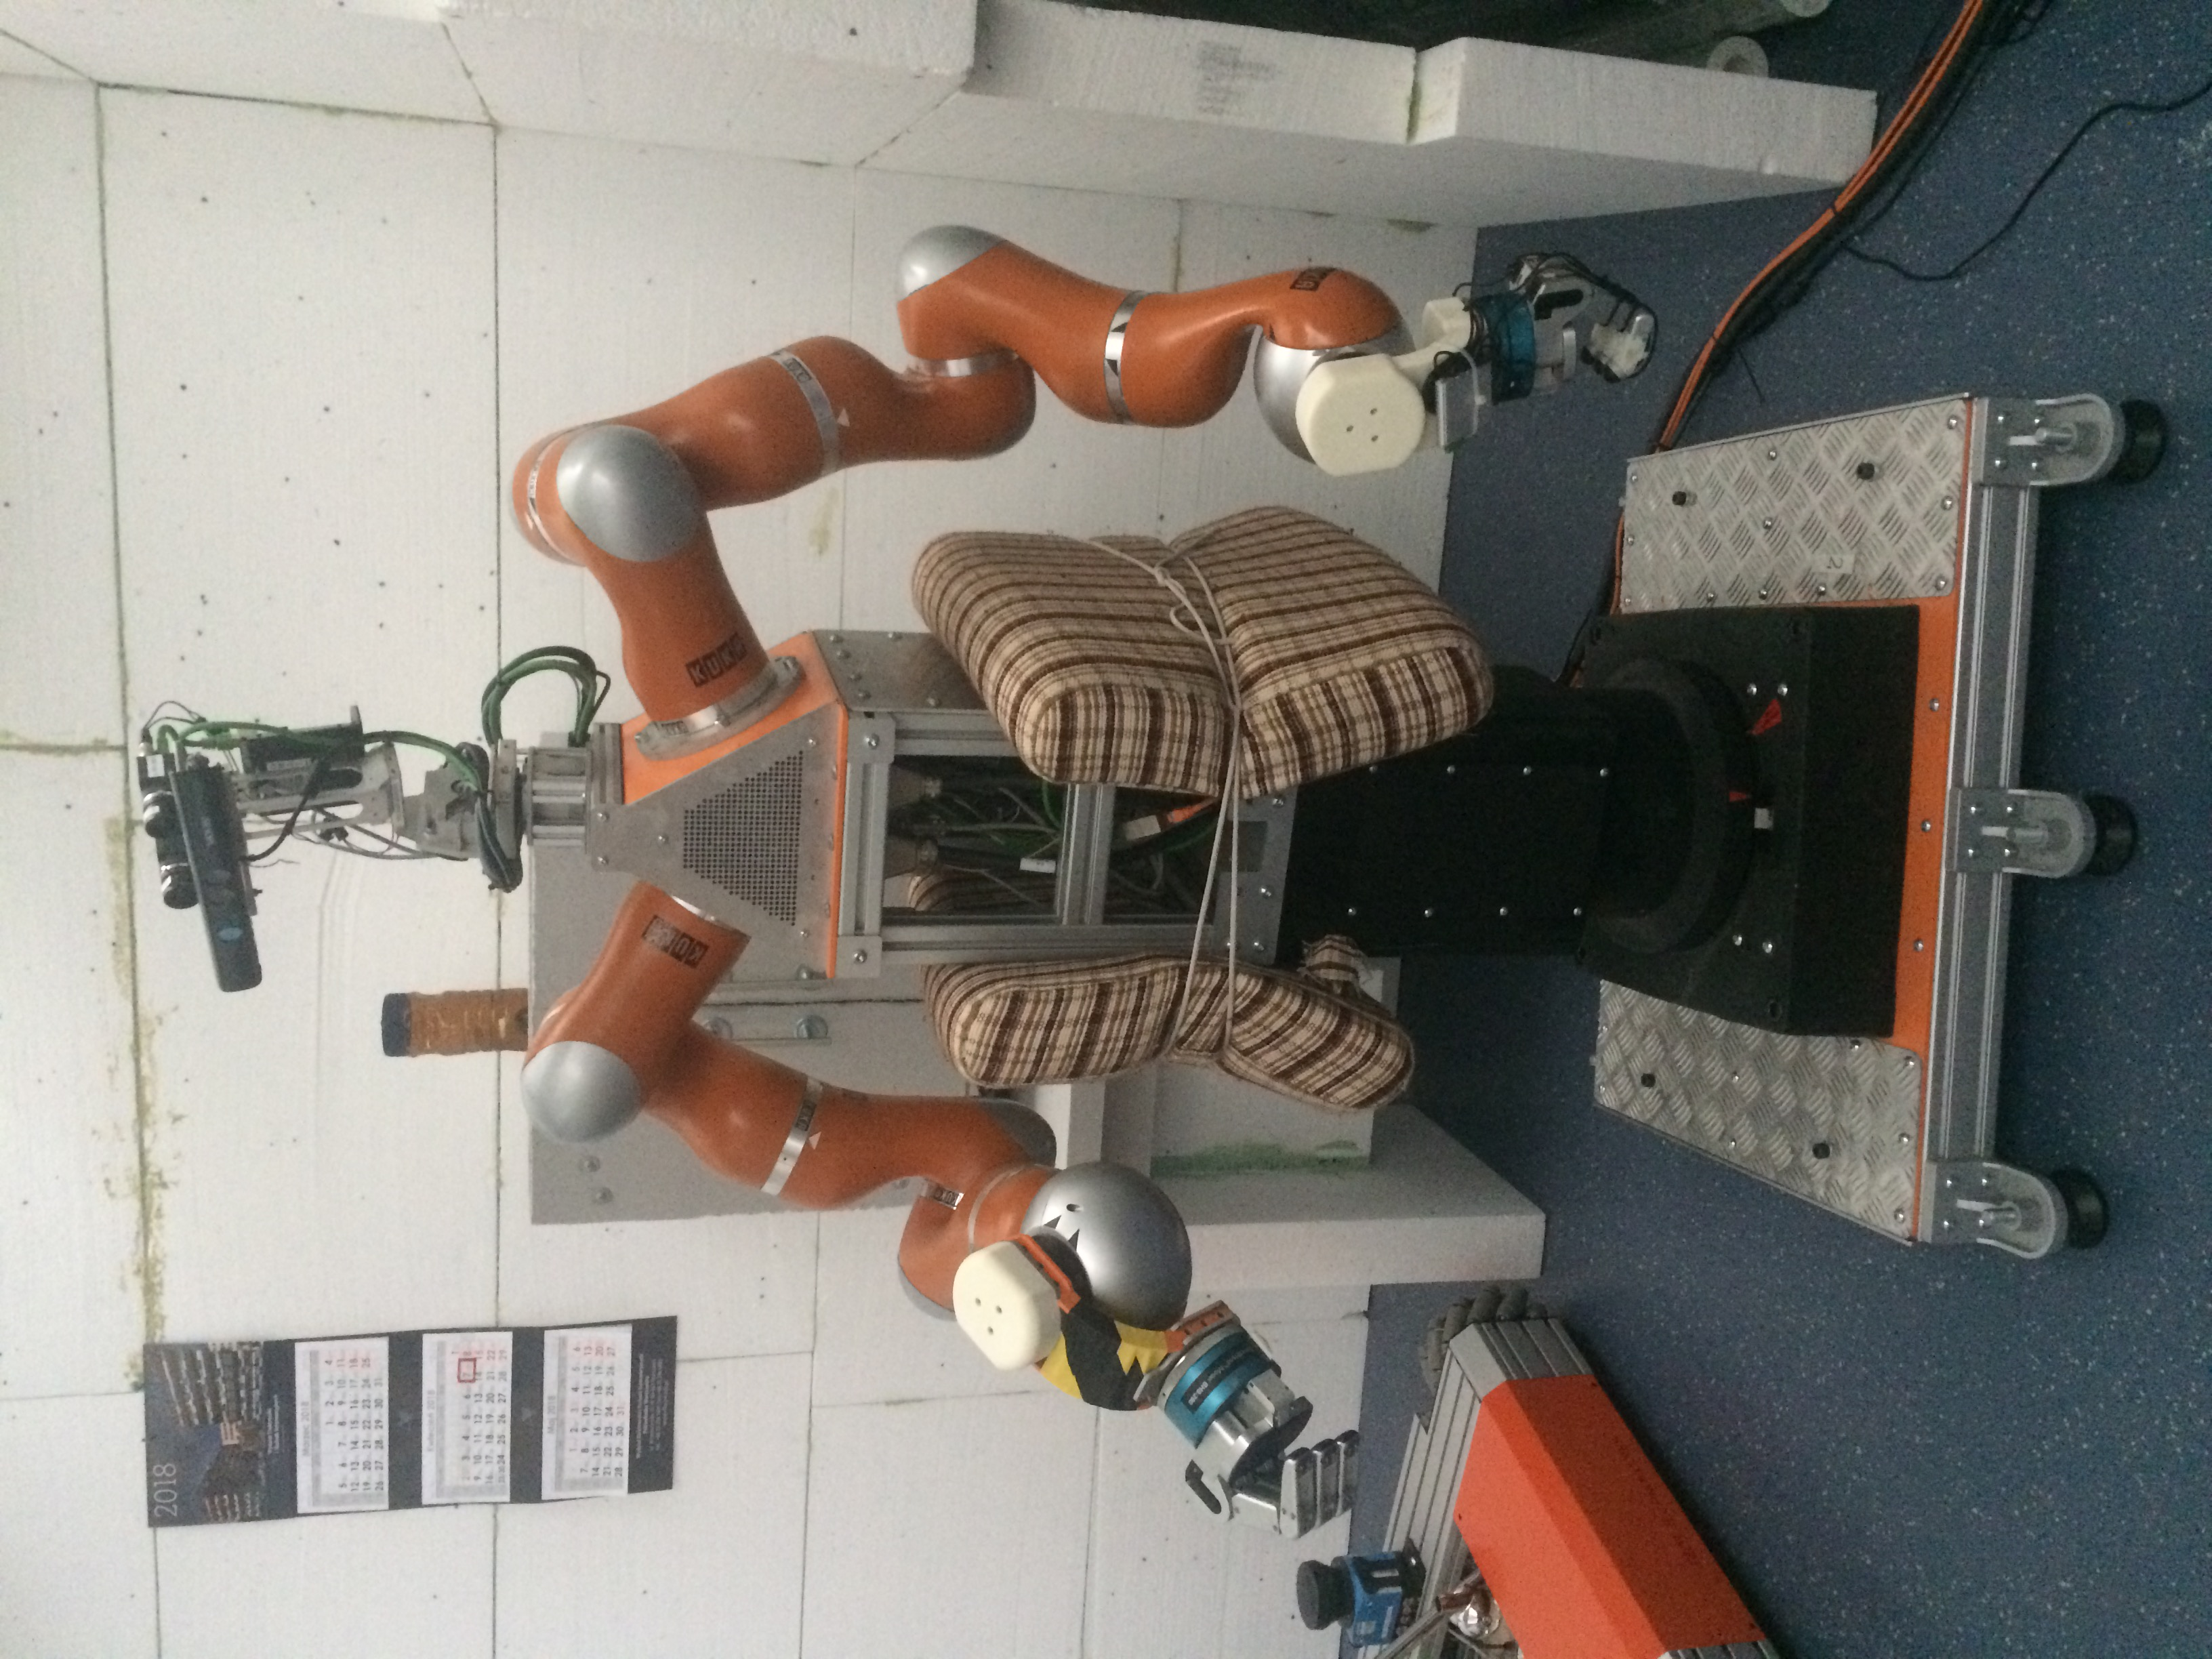
\includegraphics[width=\textwidth, angle =-90]{velma}
		\caption{Robot usługowy Velma}
		\label{fig:velma}
    \end{subfigure}
    ~ %add desired spacing between images, e. g. ~, \quad, \qquad, \hfill etc.
      %(or a blank line to force the subfigure onto a new line)
    \begin{subfigure}[b]{0.3\textwidth}
    	\centering
        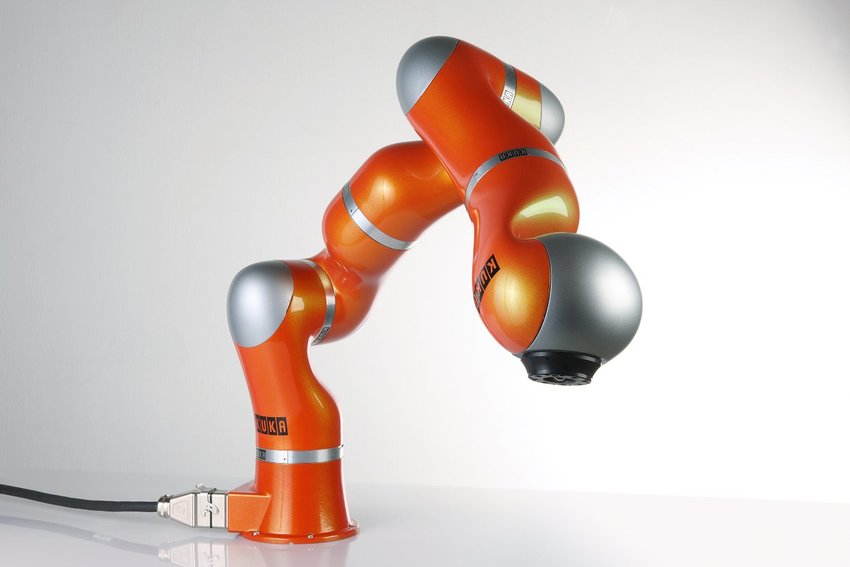
\includegraphics[width=\textwidth]{lwr}
		\caption{Ramię LWR \cite{lwr}}
		\label{fig:lwr}
    \end{subfigure}
    ~ %add desired spacing between images, e. g. ~, \quad, \qquad, \hfill etc.
    %(or a blank line to force the subfigure onto a new line)
    \begin{subfigure}[b]{0.3\textwidth}
    	\centering
		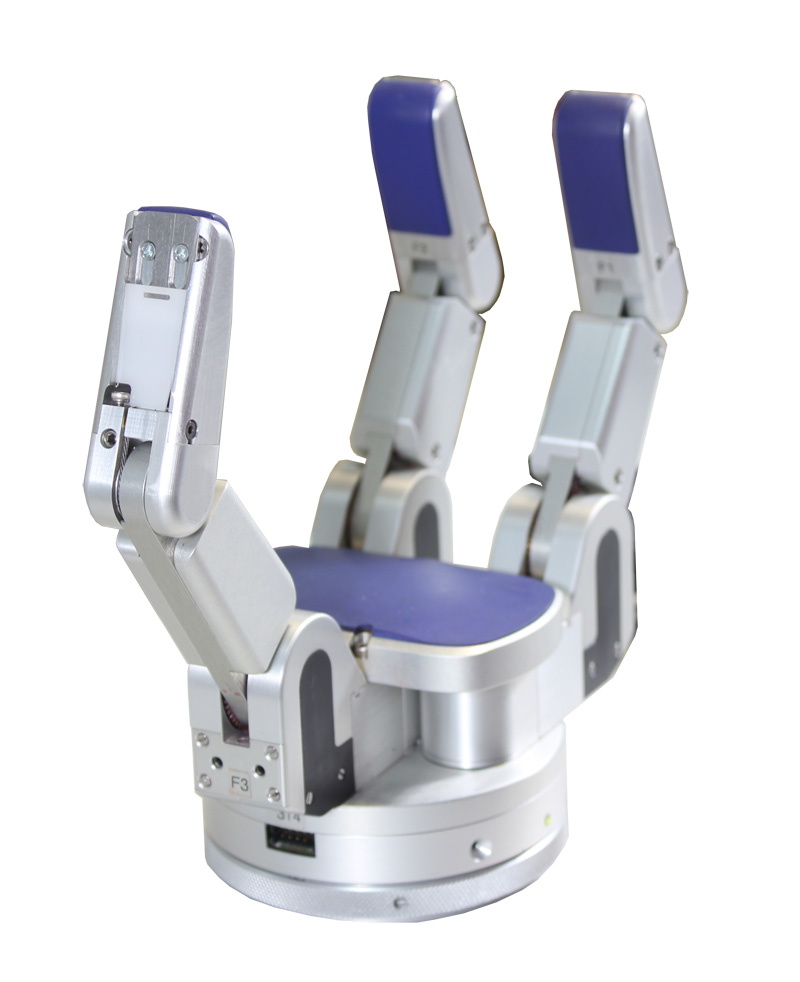
\includegraphics[width=0.6\textwidth]{icon}
		\caption{Chwytak Barretta\cite{barrett}}
		\label{fig:barrett}
    \end{subfigure}
    \caption{Podzespoły robota}\label{fig:parts}
	\end{figure}

	\begin{figure}[H]
		\centering
		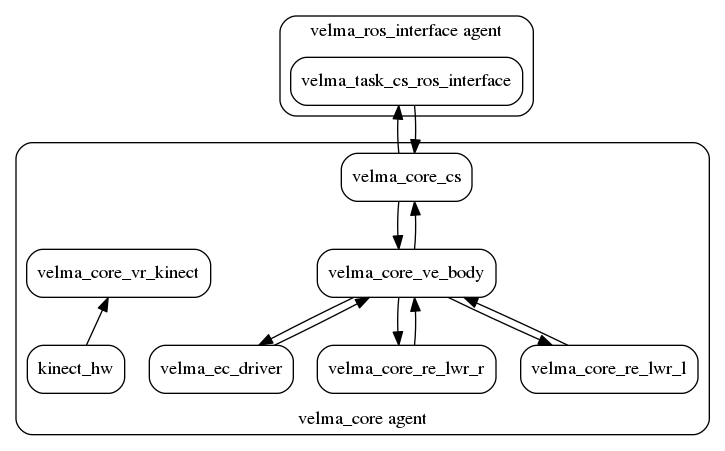
\includegraphics[width=0.8\linewidth]{agenty}
		\caption{Agentowa struktura oprogramowania \cite{velma}}
		\label{fig:agenty}
	\end{figure}

	\section{Koncepcja rozwiązania}
	Obiekt można identyfikować przetwarzając dane z czujnika FTS. W eksperymencie prowadzonym w trakcie ruchu należy uwzględnić siłę bezwładności. Wprowadza to dodatkowe utrudnienie do obliczeń ale pozwala na uzyskanie modelu który opisuje bezwładność. W celu uzyskania dokładnego modelu należy brać pod uwagę wielokrotne odczyty. Obiekt może się zmieniać w czasie. Parametru modelu muszą być aktualizowane na bieżąco. Wartą uwagi jest sytuacja gdy robot właśnie chwyta obiekt lub go upuszcza. Model powinien być czuły na tego typu gwałtowne zdarzenia. Model powinien zawierać informacje o: parametrach środka ciężkości przedmiotu, parametrach bezwładności oraz o masie obiektu.

	Metoda kompensacji powinna pobierać informacje z modelu obiektu i na podstawie tego modelu dodawać odpowiednie momenty do prawa sterowania robota. Z powodów opisanych we wprowadzeniu, rozwiązanie oparte na algorytmach niwelujących uchyb nie są pożądane Najrozsądniejszym rozwiązaniem wydaje się dopisanie odpowiednich momentów sił do prawa sterowania robota w oparciu o uzyskany model chwyconego obiektu i znany model ramienia. Przy zastosowaniu ograniczeń całkowania można próbować wykorzystać algorytmy minimalizujące uchyb. Badania warto rozwinąć o rozważania na temat regulacji adaptacyjnej.

	\section{Plan prac}
	\begin{itemize}
		\item Przegląd literatury
		\item Poszerzenie wiedzy poprzez uczęszczanie na przedmioty TST, AMO, MORO
		\item Zapoznanie ze sterownikiem robota Velma
		\item Projekt końcowych testów
		\item Koncepcja postaci modelu i uzyskania jego parametrów
		\item Koncepcja wyliczania potrzebnego momentu kompensującego grawitację
		\item Implementacja uproszczonego symulatora sterowania impedancyjnego
		\item Testy rozwiązania w uproszczonym środowisku symulatora
		\item Testy i eksperymenty rozwiązania w środowisku pełnego symulatora
		\item Testy rozwiązania w środowisku rzeczywistym
	\end{itemize}


	\bibliographystyle{unsrt}
	\bibliography{bibliography}

\end{document}